\documentclass{article}
\usepackage[utf8]{inputenc}
\usepackage{amsmath}
\usepackage{graphicx}
\usepackage{subcaption}
\usepackage{hyperref}
\addtolength{\oddsidemargin}{-0.625in}
\addtolength{\evensidemargin}{-0.625in}
\addtolength{\textwidth}{1.5in}
\addtolength{\topmargin}{-1in}
\addtolength{\textheight}{1.5in}
\title{A/B Testing and its Pitfalls}
\author{Alan Liang}
\date{May 2018}

\begin{document}
\maketitle
\section{A/B Testing}
A/B testing is a controlled experiment that compares two variants of a webpage by randomly assigning visitors to one version or the other, and measuring the relevant results.
For example, to test the click-through-rate of a certain link, a simple A/B test could be to see if a button or a banner hyperlink is more effective in getting users to click on the webpage.
\\
Companies often evaluate the effectiveness of new features and designs through A/B testing procedures on the user, and most often the users do not notice that they are being tested on.
\\
The effects of A/B testing are sometimes subtle yet huge.
Below is an example that highlights the importance yet subtleness of A/B testing: one of the versions has a 90\% decrease in sales over the other one. 
Guess which one; it surely isn't easy to tell:
\begin{figure}[h!]
  \centering
  \begin{subfigure}[b]{0.7\linewidth}
    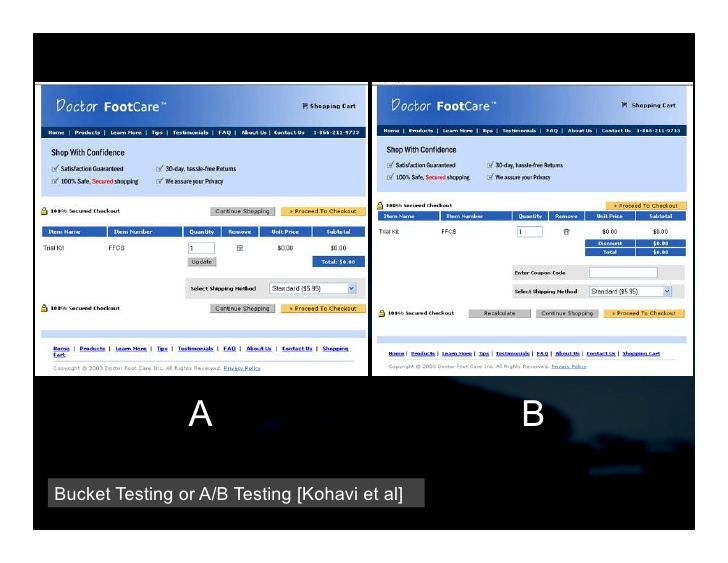
\includegraphics[width=\linewidth]{ABtesting-example.jpg}
    \caption{Which version has a 90\% decrease in sales?}
  \end{subfigure} 
\end{figure}
It turns out that the right version has a 90\% decrease. 
The culprit? The extra coupon code.
Users, after seeing this, would be discouraged to purchase or go off searching for a coupon code online, and forget about their shopping. 

\section{Procedure of A/B Testing}
Generally, A/B testing works as follows:
\begin{enumerate}
	\item Develop a new feature or new variant of a webpage, define the outcome metric, and hypothesize the causal effect of the new feature on the metric.
	\item When a user visits the webpage, randomly assign them to either the A or B variant of the webpage and measure the outcome variables for each.
	\item  After the experiment is over, conduct a p-value test to determine if the results are \textit{statistically significant}.
\end{enumerate}
This procedure of itself isn't too complicated, but there are a few things to be careful of when doing A/B Testing!

\section{Pitfalls of A/B Testing}
Both pitfalls of A/B testing below are from being able to find trends or statistically significant results in noise. 
\subsection{Multiple Comparisons}
From Data 8, we know that the p-value means how likely the observed statistic were to happen assuming the null hypothesis were to be true.
If our p-value cutoff was 0.05, then even if the null hypothesis were, 5\% of the time we would see a statistically significant result that would cause us to reject the null.
This means that if we conducted 20 trials of the same experiment, we can expect to see a statistically significant result even if the null hypothesis were true.
\\
This idea is at the heard of the multiple comparisons problem.
For one specific A/B test, if we were to compare 20 different outcome variables or metrics, it would be just like running 20 different tests; one of them is bound to end up to being statistically significant.
\\ 
For example, say we had web traffic results from 1 webpage and split the results into 2 and pretend we had an A/B test results, so that the null hypothesis is true as the underlying distribution is the same.
If we were to measure the difference in 1 outcome variable such as time spent on page, there is a 1 in 20 chance that it is statistically significant. 
However, if we were to use these results to compare another 19 variables, we should expect to see some statistically significant difference between the 2 groups.
\\
The takeaway is that we cannot compare multiple hypotheses simultaneously from the same A/B test results. 
Instead, we should try to limit the number of comparisons we make: we should only be focused on one primary outcome variable.

\subsection{Sequential Hypothesis Testing}
Say you conduct an A/B test and monitor the results daily. 
On anyday, if the cumulative results up to that day are statistically significant, then you stop the experiment.
\\
Often, we are tempted to do this due to cost or time constraints: running an A/B test may not be cheap. 
In addition, if the initial results appear to be promising, why not just directly implement it? 
\\
The problem with this is that you are more likely to find statistically significant results by peaking more times. 
Why? 
Consider the p-value of a coin over time, if we flipped it once every day and measured its p-value of it being a fair coin.
\\
\begin{figure}[h!]
  \centering
  \begin{subfigure}{0.4\linewidth}
    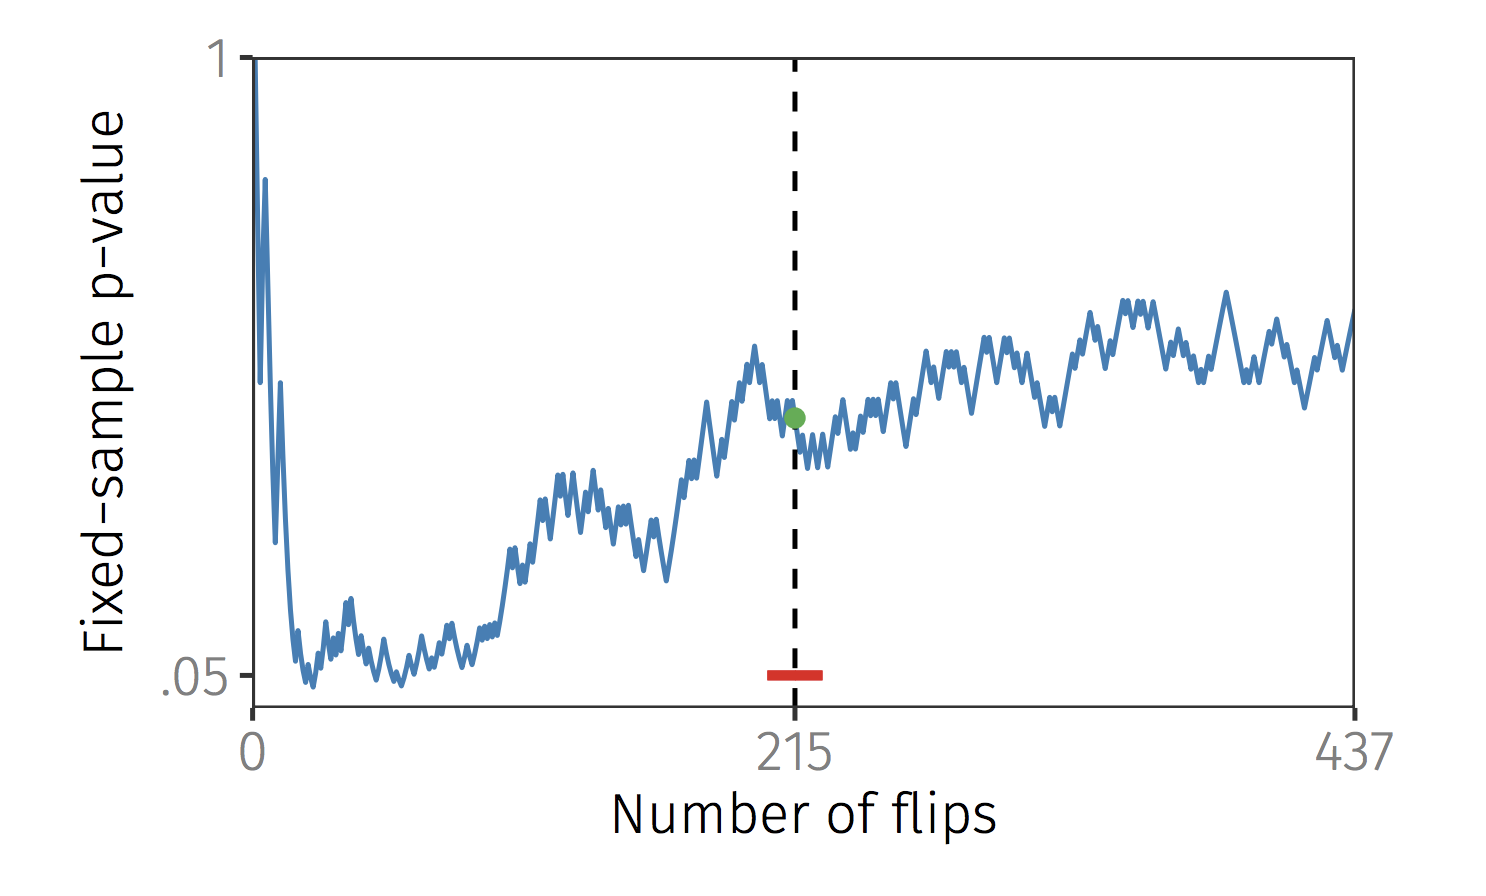
\includegraphics[width=\linewidth]{Sequential.jpg}
  \end{subfigure} 
\end{figure}
\\
Notice that around the 8th flip, our p-value dips below 5\%. 
This means that if we monitored the p-value daily, on the 8th day we would see a statistically significant result and stop the experiment, even if the coin was fair. 
Sequential testing increases the probability of seeing a faulty statistically significant result under the null hypothesis.
\\ 
The easy solution to sequential hypothesis testing is to not peek at the results. 
\\
Or we could factor in sequential hypothesis testing into our null results and conduct simulation based sequential p-value testing (note that this material was not covered in lecture. You can learn more about it \underline{\href{http://www.ds100.org/sp18/assets/lectures/lec28/28-randomized-experiments-ab-testing.pdf}{here}}).
Say we stopped on the 8th day. 
In this case, we would essentially recreate via simulations the null hypothesis, assuming that we peeked every day in all the simulations, and record how many of the simulations would also have recorded a statistically significant result on any of the days up to the 8th day.
Then, we would see the frequency of how many of the null simulations produced statistically significant results and would have stopped the experiment up to the 8th day, out of all the simulations.
This frequency value, which measures how likely our observed results were to appear statistically signifiicant happen under the null hypothesis, is exactly the p-value.
If this value is above 5\%, then the results are likely not statistically significant.


\end{document}